\thispagestyle{empty}
\begin{center}
%{\Huge A BOOK}
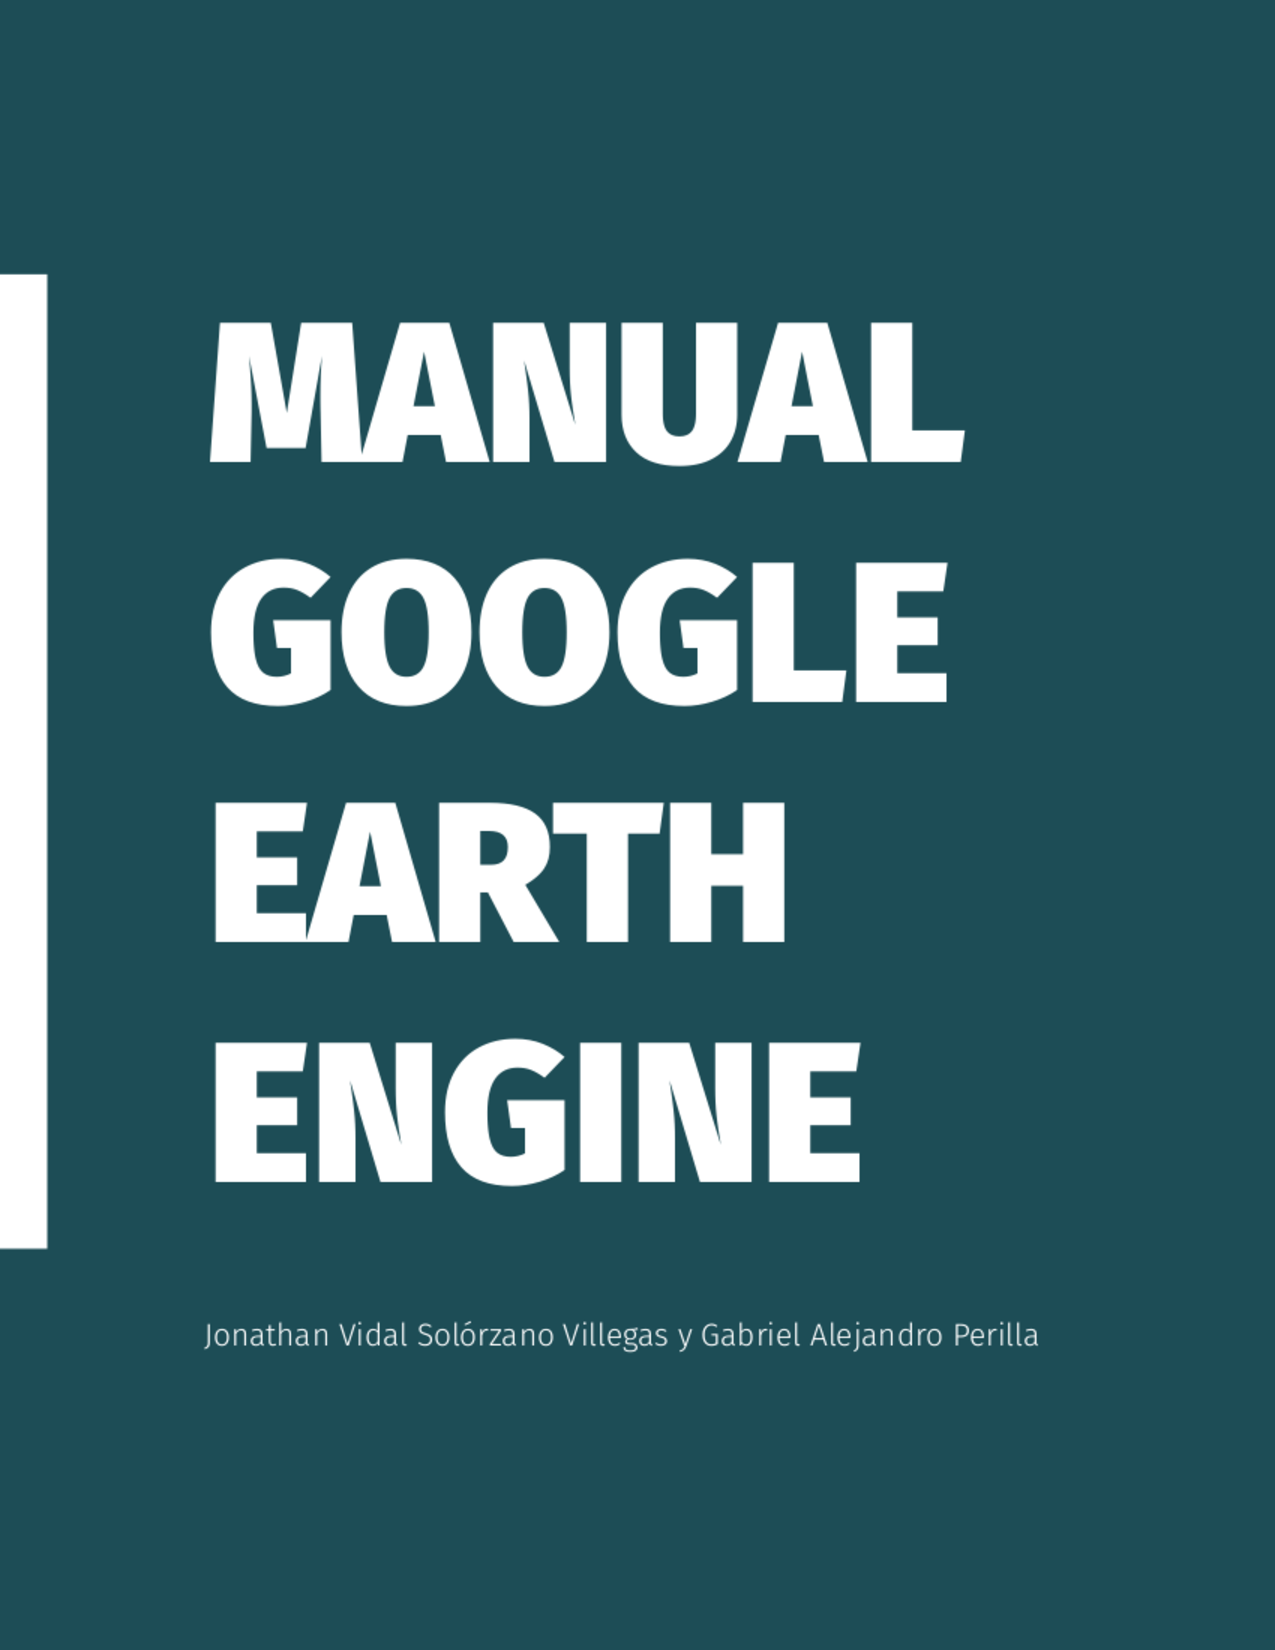
\includepdf{Img/Portada.pdf}
%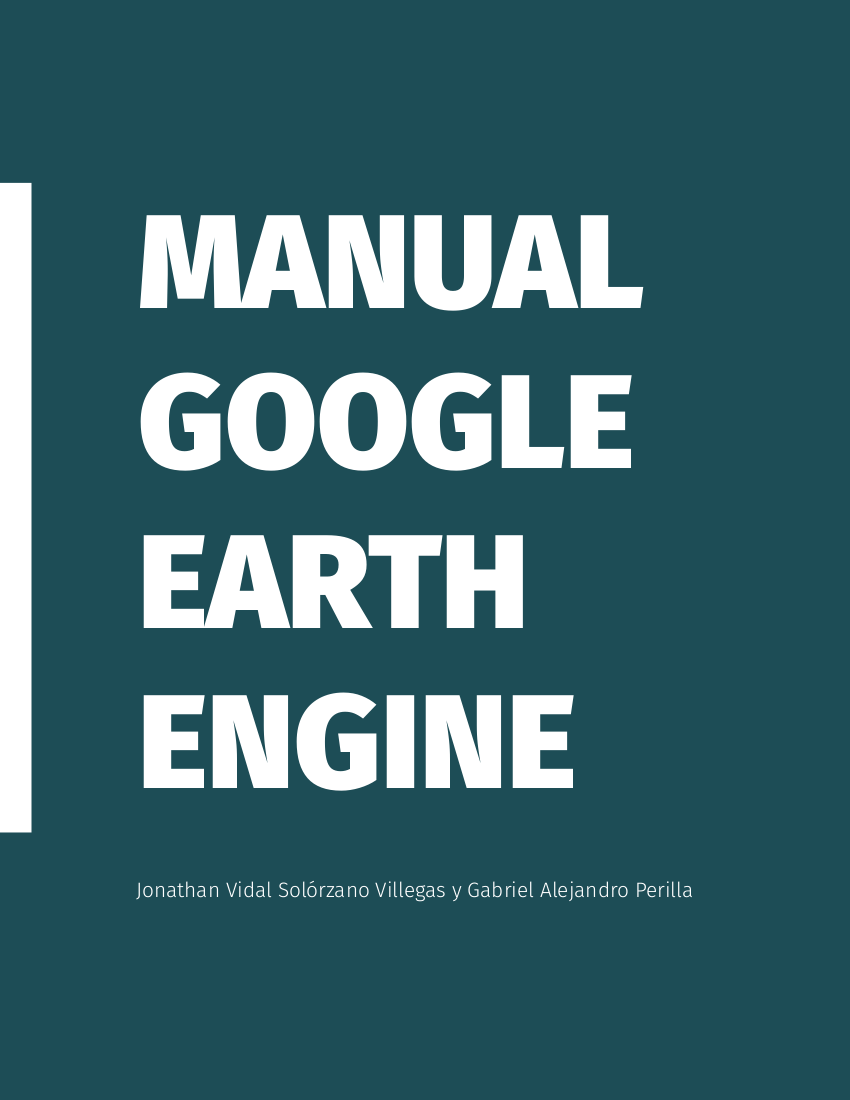
\includegraphics{Img/Portada.png}
%{\huge by Jonathan Vidal Solórzano Villegas y Alejandro Perilla Suárez}
\end{center}

% Título
\newpage
\topskip0pt
\vspace*{\fill}
\begin{center}
\LARGE{Cómo usar Google Earth Engine y no fallar en el intento}
\end{center}
\vspace*{\fill}

% Instituciones
\newpage

\topskip0pt
\vspace*{\fill}
\begin{center}
\large{Centro de Investigaciones en Geografía Ambiental}
\linebreak
\large{Universidad Nacional Autónoma de México}
\linebreak
\large{Instituto de Investigación de Recursos Biológicos Alexander von Humboldt}
\end{center}
\vspace*{\fill}

% Logos
\newpage

\topskip0pt
\vspace*{\fill}
\begin{center}
\LARGE{Cómo usar Google Earth Engine y no fallar en el intento}
\linebreak
\linebreak
\large{Jonathan Vidal Solórzano Villegas y Gabriel Alejandro Perilla Suárez}
\end{center}
\vspace{15mm}
\setlength{\columnsep}{40pt}
\begin{multicols}{2}
%\noindent
    \begin{Figure}
    \centering
    
\includegraphics[width=0.7\linewidth]{Img/unam}
    %\captionof{figure}{my caption of the figure}
    \end{Figure}
    \centering Universidad Nacional Autónoma de México
    %\columnbreak
    \begin{Figure}
    \centering
    
\includegraphics[width=0.7\linewidth]{Img/humb}
    %\captionof{figure}{my caption of the figure}
    \end{Figure}
    \centering Instituto de Investigación de Recursos Biológicos Alexander von Humboldt 
\end{multicols}
\vspace*{\fill}

% Página legal
\newpage

\topskip0pt
\vspace*{\fill}
\begin{center}
    \begin{blackbox}
        {\footnotesize \textbf{Catalogación en la publicación UNAM. Dirección General de Bibliotecas y Servicios Digitales de Información}

            \textbf{Nombres:} Solórzano Villegas, Jonathan Vidal, autor. | Perilla Suárez, Gabriel Alejandro, autor.  

            \textbf{Título:} Cómo usar Google Earth Engine y no fallar en el intento / Jonathan Vidal Solórzano Villegas y Gabriel Alejandro Perilla Suárez.

            \textbf{Descripción:} Primera edición. | Morelia, Michoacán de Ocampo : Universidad Nacional Autónoma de México, Centro de Investigaciones en Geografía Ambiental ; Bogotá, Colombia : Instituto de Investigación de Recursos Biológicos Alexander von Humboldt, 2022.  
            
            \textbf{Identificadores:} LIBRUNAM 2167765 (libro electrónico) | ISBN (libro electrónico) (UNAM) | ISBN (libro electrónico) (Colombia).    
            
            \textbf{Temas:} Computación en nube. | Sistemas de información geográfica. | Almacenamiento de datos. | Google Earth Engine (Programa para computadora). 
            
            \textbf{Clasificación:} LCC QA76.585 (libro electrónico) | DDC 004.6782—dc23}
        
    \end{blackbox}
    %\begin{blackbox}
    %    {\footnotesize Solórzano Villegas, Jonathan Vidal y Perilla Suárez, Gabriel Alejandro
%
    %    \quad Cómo usar Google Earth Engine y no fallar en el intento. – México: Universidad Nacional Autónoma 
%            
   %     \quad de México e Instituto de Investigación de Recursos Biológicos Alexander von Humboldt.
%
    %    \quad 196 p, : il. col. ; 27 cm.
%
     %   \quad Bibliografía: p. 193 – 195
%
      %  \quad ISBN obra digital México: xxx-xxx-xxxx-xx-x; ISBN obra digital Colombia: xxx-xxx-xxxx-xx-x.
%
       % \quad 1. Procesamiento en la nube – Información geoespacial 2. Programación}
%        
        %\begingroup
        %    \fontfamily{lmss}\fontsize{10}{12}\selectfont
        %    Solórzano Villegas, Jonathan Vidal y Perilla Suárez, Gabriel Alejandro
        %    \quad Cómo usar Google Earth Engine y no fallar en el intento. – México: Universidad Nacional Autónoma 
        %    \quad de México e Instituto de Investigación de Recursos Biológicos Alexander von Humboldt.
        %    \quad 196 p, : il. col. ; 27 cm.
        %    \quad Bibliografía: p. 193 – 195
        %    \quad ISBN obra digital México: xxx-xxx-xxxx-xx-x; ISBN obra digital Colombia: xxx-xxx-xxxx-xx-x.
        %    \quad 1. Procesamiento en la nube – Información geoespacial 2. Programación
        %\endgroup
%    \end{blackbox}
\end{center}

\setlength{\columnsep}{25pt}
\begin{multicols*}{2}
    \raggedcolumns
    {\scriptsize Este libro ha sido arbitrado por pares académicos y fue posible gracias al Proyecto PE117519-Programa de Apoyo a Proyectos para la Innovación y Mejoramiento a la Enseñanza (PAPIME), DGAPA, UNAM. 
    \linebreak Este trabajo tiene algunos derechos reservados según lo especifica la licencia internacional {\it Creative Commons Attribution Non Commercial Share Alike 4.0 (CC-BY-NC-SA)}, la cual puede consultar en \href{https://creativecommons.org/licenses/by-nc-sa/4.0/legalcode.es}{https://creativecommons.org/licenses/by-nc} \href{https://creativecommons.org/licenses/by-nc -sa/4.0/legalcode.es}{-sa/4.0/legalcode.es}
    \linebreak
    \linebreak
    %\vfill
    %\medskip
    \begingroup
        
\includegraphics[height=28pt]{Img/license}
    \endgroup
    \newline Diseño editorial: Jonathan Vidal Solórzano Villegas y Laura Perilla Suárez (\href{https://behance.net/lauuuuperilla}{behance.net/lauuuuperilla}).
    \newline Imagen en portada y la contraportada: 20181227T151659\_ 20181227T151707\_19PBN (Sentinel-2) modificada de datos Copernicus Sentinel-2 registrados en 2018/12/27. 
    \newline Imágenes: todas las imágenes fueron creadas por los autores, los screenshots pueden contener pequeñas anotaciones con fines aclaratorios para los usuarios, estas imágenes cumplieron con las pautas y uso de marca de Google, de modo que aplican los términos y condiciones de marca registradas. 
    \newline Todos los nombres de marcas y productos mencionados en esta obra están sujetos a la protección de marcas comerciales, marcas o patentes y las marcas comerciales o marcas comerciales registradas por sus respectivos titulares. 
    El uso de nombres de marca, nombres de productos, nombres comunes, nombres comerciales, descripciones, etc. incluso sin una marca particular en este trabajo no puede de ninguna manera interpretarse en el sentido de que dichos nombres pueden considerarse sin restricciones con respecto a la legislación sobre marcas comerciales y protección de marcas y, por lo tanto, podrían ser utilizados por cualquiera.
    \linebreak
    \newline Revisión académica: Andrea Pamela Flores, Victoria Nazarena Guzmán, Sandra Lucía Hernández Zetina, Xanat Antonio Némiga. \hspace*{\fill}
    \linebreak
    \newline Primera edición, agosto 2022. Morelia - México, Bogotá - Colombia.  
    D. R. © 2022 Universidad Nacional Autónoma de México 
    Ciudad Universitaria sin número, Coyoacán, C.P. 04510, Ciudad de México, México.
    www.unam.mx
    \newline Centro de Investigaciones en Geografía Ambiental (CIGA, UNAM) 
    Antigua carretera a Pátzcuaro 8701, Exhacienda de San José de la Huerta, C.P. 58190, Morelia, Michoacán de Ocampo, México.
    publicaciones.ciga.unam.mx
    \newline Instituto de Investigación de Recursos Biológicos
    Alexander von Humboldt, Calle 72 no 12-65, piso 7, Bogotá,
    Colombia. http://www.humboldt.org.co/es/
    comunicaciones@humboldt.org.co
    \newline ISBN obra digital Colombia: xxx-xxx-xxxx-xx-x \hspace*{\fill}
    \newline ISBN obra digital México: xxx-xxx-xxxx-xx-x \hspace*{\fill}
    \linebreak
    \newline Esta edición y sus características son propiedad de la Universidad Nacional Autónoma de México y del Instituto de Investigación de Recursos Biológicos Alexander von Humboldt. Prohibida la reproducción total o parcial por cualquier medio sin la autorización escrita del titular de los derechos patrimoniales.}
\end{multicols*}
\vspace*{\fill}

% Para hacer el título por default después
\let\maketitle\oldmaketitle
\maketitle